\documentclass[letterpaper, 10 pt, conference]{ieeeconf}

\usepackage{algorithm}
\usepackage[noend]{algpseudocode}
\usepackage{bm}

\usepackage{amsfonts}
\usepackage[pdftex]{graphicx}
\usepackage{comment}

\usepackage{caption}
\usepackage{subcaption}

%\usepackage{amsthm}
\newtheorem{thm}{Theorem}
\newtheorem{lem}{Lemma}
%\newtheorem{asmp}{Assumption}
%\newtheorem{defn}{Definition}
%\newtheorem{clm}{Claim}

\IEEEoverridecommandlockouts                              % This command is only needed if 
                                                          % you want to use the \thanks command

\overrideIEEEmargins                                      % Needed to meet printer requirements.

\title{\LARGE \bf
Homotopy-aware RRT$^{*}$ : Homotopy-based sampling-based optimal path planning
}

\author{
Daqing Yi, Michael A. Goodrich and Kevin D. Seppi
\thanks{Daqing Yi, Michael A. Goodrich and Kevin D. Seppi are with Department of Computer Science, Brigham Young University, Provo, UT, 84604, USA.
{\tt\small daqing.yi@byu.edu, mike@cs.byu.edu, kseppi@cs.byu.edu} }
}

\begin{document}


\maketitle
\thispagestyle{empty}
\pagestyle{empty}


%%%%%%%%%%%%%%%%%%%%%%%%%%%%%%%%%%%%%%%%%%%%%%%%%%%%%%%%%%%%%%%%%%%%%%%%%%%%%%%%
\begin{abstract}
Because the topology factor is difficulty to abstract for a task planner, it is often ignored in modeling the problems of optimal motion planning, especially when it is not a hard constraint.
In this paper, we propose HA-RRT$^{*}$, a homotopy-aware RRT$^{*}$, that explores the planning space for optimal solutions with the consideration of the topology of the paths.
When the task planner has a clear will on the topology of the paths, the homotopy-aware RRT$^{*}$ could utilize this information as prior to reduce the working space of the optimal search.
When the task planner has a vague will on the topology of the paths, the homotopy-aware RRT$^{*}$ could help the planner find the optimal solutions that satisfies his/her intent.


\end{abstract}

\begin{comment}
six pages
\end{comment}

%%%%%%%%%%%%%%%%%%%%%%%%%%%%%%%%%%%%%%%%%%%%%%%%%%%%%%%%%%%%%%%%%%%%%%%%%%%%%%%%
\section{INTRODUCTION}
\label{sec:intro}

One of the most important targets of robotic path planning is the optimality to some level.
%The most popular focus on the robotic path planning is optimality.
This depends on an assumption that the problem has been well modeled.
Thus, the solution 
In planning the robot's motion in a task, the intent of the task supervisor is usually modeled into single objective~\cite{6974170} or multiple objective optimization~\cite{yi2014supporting}.
The generated path is a solution that optimizes the given objectives, for example, minimizing the Euclidean distance.
There exist plenty of other human intents that are hard to be modeled using measurable metrics.
A class of them can be relevant with the ``shape'' of the planned path, especially in environments with complex obstacles.
For example, the human supervisor would like the robot reaching a target in the shortest time while passing through some locations.
The most common solution is defining via points as a constraint for the path planning problem.
However, sometimes this intent is only a preference instead of a hard constraint.

\emph{Homotopy} is imported to model the inherent topological similarity of the paths.
Given two paths, if one can be deformed into the other without encroaching any obstacle, they are said to be \emph{homotopic}~\cite{Hernandez201544}.
This leads to a \emph{homotopy class}, in which any two paths are homotopic.
The homotopy of the paths can help to model the human intent, which can be applied to four levels of planner's intent.
\begin{enumerate}
\item \emph{The planner has a clear intent of how the topology should be.}
The objective becomes only finding the optimal solution in the paths of this homotopy class.
The homotopy class becomes the constraint of the problem~\cite{Hershberger199463}.
This homotopy class could be defined from a human initialized reference path.
\item \emph{The planner expects the paths through some regions.}
With the via-regions given, several homotopy classes that across those regions could be obtained.
In this case, the homotopic constraint becomes several homotopy classes instead of only one.

\item \emph{The planner could tell the preference of different homotopy classes.}
With the preference of different homotopy classes, the homotopy classes could form a new objective as discrete variable.
We could firstly find the non-dominant solutions.
Thus the planner could figure out one from the Pareto optimal paths.
\item \emph{The planner could not tell the preference of different homotopy classes.}
If the task supervisor has a weak opinion on the topology of the path, the planning algorithm can provide the best solution of each homotopy class to the supervisor.
The supervisor can then select one that satisfy his/her intent.
\end{enumerate}

In this paper, we propose a homotopy-aware RRT$^{*}$ that awares the homotopy class while exploring the planning space.
It could assist the planner finding the intended optimal path in considering the homotopy.

\section{Related work}
\label{sec:related_work}

\subsection{Homotopy-based Path Planning}

Homotopy-based path planning depends on the determination of the homotopy equivalence of two paths, which is usually computationally expensive.

Voronoi diagram is naturally introduced to assist determining the homotopy classes, but it shows limitation on finding some paths in some cases~\cite{banerjee2013framework}.
By algebraic topology, the path of same homotopy class can be determined by using orientable band~\cite{Hershberger199463}.
Semi-algebraic cuts are used to converting the path into ``word'' so that the homotopic equivalence can be compared~\cite{Grigoriev:1998:PAS:281508.281528}.
The Cauchy Integral theorem has been introduced to determine homotopy class by marking the positions in the obstacles as undefined~\cite{AAAI101920}.

\subsection{Homotopy RRT / PRM}

By homotopic redundancy, the paths from PRM could be compared by the homotopy classes~\cite{1041613}.
By dividing the space using the rays crossing each obstacle, reference frames could be used to represent the paths into canonical sequences~\cite{Hernandez201544}.

\subsection{Bidirectional RRT}

Bidirectional RRT has been introduced to accelerate the exploration process while the optimality is still preserved~
\cite{Jordan.Perez.ea:CSAIL13}~\cite{starek2014bidirectional}.

With two trees exploring from two directions, we can have the optimal cost-to-go and the optimal cost-to-arrive at different position.
This guarantee the optimality search with the homotopical constraint.
We introduce the homotopy-aware bidirectional RRT$^{*}$ to support different level of intent on topology from the planner.

\section{Homotopy-aware RRT$^{*}$}
\label{sec:algorithm}

\begin{algorithm}[hbtp]
	\begin{algorithmic}[1]
		\State $ \bm{R} = \emptyset $
		\For{\textbf{each} $ B_{k} \in \bm{B} $ }
			\State $ b_{k} $ $ \leftarrow $ Sample from $ B_{k} $
			\State $ \bm{b} \leftarrow \bm{b} \cup b_{k} $
		\EndFor
		\While{ $ \exists b_{k}, b_{k'} , c \in $ \Call{Line}{ $ b_{k}, b_{k'} $ } }
			\State $ c \leftarrow  $ Sample from $ \bm{X}_{free} $
		\EndWhile
		\For{\textbf{each} $ b_{k} \in \bm{b} $ }
			\State $ \alpha_{k} \leftarrow $ \Call{Ray}{ $ b_{k}, c - b_{k} $ }
			\State $ \beta_{k} \leftarrow $ \Call{Ray}{ $ b_{k}, b_{k} - c $ }
			\State $ \bm{\alpha} \leftarrow \bm{\alpha} \cup \alpha_{k} $
			\State $ \bm{\beta} \leftarrow \bm{\beta} \cup \beta_{k} $			
		\EndFor
		\For{\textbf{each} $ \alpha_{k} \in \bm{\alpha} $}
			\State $ \{ \alpha_{k_{m}} \} \leftarrow $ \Call{Intersect}{$ \alpha_{k}, \bm{B} $}
			\State $ \bm{R} \leftarrow \bm{R} \cup \{ \alpha_{k_{m}} \} $
		\EndFor
		\For{\textbf{each} $ \beta_{k} \in \bm{\beta} $}
			\State $ \{ \beta_{k_{m}} \} \leftarrow $ \Call{Intersect}{$ \beta_{k}, \bm{B} $}
			\State $ \bm{R} \leftarrow \bm{R} \cup \{ \beta_{k_{m}} \} $
		\EndFor
		\Return $ \bm{R} $
	\end{algorithmic}
	\caption{ \textsc{InitRefFrames} ($ \bm{X}_{free} , \bm{B} $) }
	\label{alg:harrt:init_ref_frames}
\end{algorithm} 

\begin{itemize}
	\item \textsc{Line}($ p_{1}, p_{2} $):
	Return a line that defined by $ p_{1} $ and $ p_{2} $.
	\item \textsc{Ray}($ p, \vec{d} $):
	Return a ray that starts from $ p $ with direction $ \vec{d}  $.
	\item \textsc{Intersect}( $ r , \bm{B} $ ):
\end{itemize}

\begin{algorithm}
	\begin{algorithmic}[1]
		\State $ i \leftarrow 0 $
		\State $ V_{s} \leftarrow \{ x_{init} \} $; $ E_{s} \leftarrow \emptyset $; $ G_{s} \leftarrow (V_{s}, E_{s}) $
		\State $ V_{g} \leftarrow \{ x_{goal} \} $; $ E_{g} \leftarrow \emptyset $; $ G_{g} \leftarrow (V_{g}, E_{g}) $
		\While{ $ i < N $ }
			\State $ G_{s} \leftarrow $ \Call{Explore}{$ G_{s}, i $}
			\State $ G_{g} \leftarrow $ \Call{Explore}{$ G_{g}, i $}
			\State $ i \leftarrow i + 1 $
		\EndWhile
		\State \Call{ExtractPaths}{$ G_{s}, G_{g} $}
	\end{algorithmic}
	\caption{HA-RRT$^{*}$ ($ x_{init} , x_{goal}  $) }
	\label{alg:harrt}
\end{algorithm}

\begin{algorithm}
	\begin{algorithmic}[1]
		\State $ x_{rand} \leftarrow $ \Call{ Sample }{$ i $} ;
		\State $ x_{nearest} \leftarrow $ \Call{Nearest}{$ G, x_{rand} $}
		\State $ x_{new} \leftarrow $ \Call{Steer}{$ x_{nearest}, x_{rand},\eta $}
		\If{ \Call{ObstacleFree}{$ x_{nearest}, x_{new} $} }
			\State $ G \leftarrow $ \Call{ Extend }{$ G, x_{new}, x_{\it nearest} $}
		\EndIf
		\Return $ G $
	\end{algorithmic}
	\caption{ \textsc{Explore}($ G, i $) }
	\label{alg:harrt:explore}
\end{algorithm}

\begin{algorithm}
	\begin{algorithmic}[1]
		\State $ V' \leftarrow V $; $ E' \leftarrow E $
		\State $ V' \leftarrow V' \cup \{ x_{new} \} $
		\State $ x_{min} \leftarrow x_{nearest} $
		\State $ X_{near} \leftarrow $ \Call{Near}{$ G, x_{new}, | V | $}
		\State $ s \leftarrow $ \Call{STR}{$x_{new}$} $ \cup $ \Call{CRF}{$ ( x_{new}, x_{near} ), \bm{B} $}
		\If{\Call{HomotopyCheck}{$ s $}}
			\For{\textbf{each} $ x_{near} \in X_{near} $ }
				\If{ \Call{ObstacleFree}{$ x_{new} , x_{near} $} }
					\State $ c' \leftarrow $ \Call{Cost}{$ x_{near} $} $ + c( $ \Call{Line}{$ x_{near}, x_{new} $} $ ) $ 
					\If{ $ c' < $ \Call{Cost}{$ x_{new} $} }
						\State $ x_{min} \leftarrow x_{near} $
					\EndIf
				\EndIf
			\EndFor
		\Else
		    \State \Return $ G' = (V', E') $ 		
		\EndIf
		\State $ E' \leftarrow E' \cup \{ ( x_{min}, x_{new} ) \} $
		\For{\textbf{each} $ x_{near} \in X_{near} \setminus \{ x_{min} \} $ }
			\If{\Call{ObstacleFree}{$ x_{new} , x_{near} $} and \Call{Cost}{$ x_{near} $} $ > $ \Call{Cost}{$ x_{new} $} + c(\Call{Line}{$ x_{new}, x_{near} $}) }
			    \State $ s \leftarrow $ \Call{STR}{$x_{new}$} $ \cup $ \Call{CRF}{$ ( x_{new}, x_{near} ), \bm{B} $}
			    \If{\Call{HomotopyCheck}{$ s $}}
					\State $ x_{parent} \leftarrow $ \Call{Parent}{$ x_{near} $}
					\State $ E' \leftarrow E' \setminus \{ ( x_{parent}, x_{near} ) \} $
					\State $ E' \leftarrow E' \cup \{ ( x_{new}, x_{near} ) \} $
					%\State \Call{STR}{$x_{near}$} $ \leftarrow $ \Call{STR}{$x_{new}$} 
					%\State \Call{STR}{$x_{near}$} $ \leftarrow $ \Call{STR}{$x_{near}$} $ \cup $ \Call{CRF}{$ ( x_{new}, x_{near} ), \bm{B} $}
				\EndIf
			\EndIf
		\EndFor
		\Return $ G' = (V', E') $ 
	\end{algorithmic}
\label{alg:harrt:extend}
\caption{ {\sc Extend } ($ G, x_{new}, x_{nearest} $) }
\end{algorithm}

\begin{itemize}
	\item \textsc{CRF}($ l, \bm{R} $):
	Returns the character that represents the crossed reference frames if any.
	\item \textsc{STR}($ x $):	
	\item \textsc{HomotopyCheck}{($ s $)}
\end{itemize}

\begin{algorithm}
	\begin{algorithmic}[1]
		\State $ V_{s,g} \leftarrow $ \Call{SameVertices}{$ G_{s}, G_{r} $}
		\State $ P \leftarrow \emptyset $
		\For{\textbf{each} $ v \in V_{s,g} $ }
			\State $ p_{s} \leftarrow $ \Call{Path}{$ v, G_{s} $}
			\State $ p_{g} \leftarrow $ \Call{Path}{$ v, G_{g} $}
			\State $ p \leftarrow $ \Call{Concatenate}{$  p_{s}, p_{g} $}
			\State $ P \leftarrow P \cup \{ p \} $
		\EndFor
		\Return $ P $
	\end{algorithmic}
	\caption{ \textsc{ExtractPaths}($ G_{s}, G_{r} $) }
	\label{alg:harrt:binding}
\end{algorithm}


\section{Analysis}
\label{sec:analysis}

\subsection{homotopic grammar}

Each path or subpath can be converted into a string, which represents a sequence of characters by crossed reference frames.
The grammar of the strings could be introduced to manage the exploration process and sort the paths into different homotopy classes.

\begin{figure}
	\centering
	\begin{subfigure}[t]{0.45\linewidth}
		\centering
		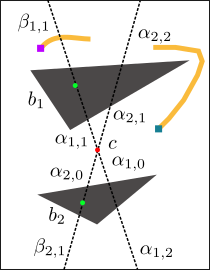
\includegraphics[width=\textwidth]{fig/feasibility}
		\caption{Feasibility}
		\label{fig:grammar:feasibility}
	\end{subfigure}  
	\begin{subfigure}[t]{0.45\linewidth}
		\centering
		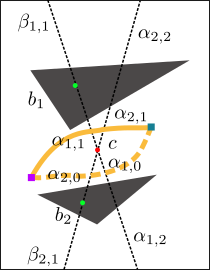
\includegraphics[width=\textwidth]{fig/equivalence}
		\caption{Equivalence}
		\label{fig:grammar:equivalence}
	\end{subfigure}
	\\
	\begin{subfigure}[t]{0.45\linewidth}
		\centering
		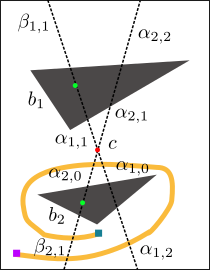
\includegraphics[width=\textwidth]{fig/recurring}
		\caption{Recurring}
		\label{fig:grammar:recurring}
	\end{subfigure}  
	\begin{subfigure}[t]{0.45\linewidth}
		\centering
		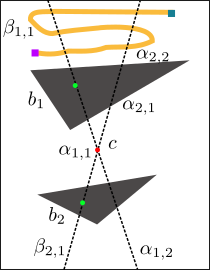
\includegraphics[width=\textwidth]{fig/repeated_pattern}
		\caption{Equivalence}
		\label{fig:grammar:repeated_pattern}
	\end{subfigure} 
	\caption{Homotopic grammar.}
	\label{fig:grammar}
\end{figure}

\begin{itemize}
\item \textbf{Feasibility}
As the reference frames are connected by the regions, a feasible string follows some grammar defined by the connectivity.

\item \textbf{Equivalence}
Some characters of the reference frames are equivalent in constructing the strings.
All the reference frames contains the center point $ c $ show this property.
The segment crossing those reference frames in any sequence belongs to same homotopy class.


\item \textbf{Recurring character}
Recurring character in a string indicates that the path goes around some obstacles and back to a visited region.


\item \textbf{Repeated pattern}
Repeated pattern shows that the path is back and forth among some regions.

\end{itemize}

\subsection{Optimality with constraint}

We can have the asymptotic optimality with the constraint of via-points.
It is stated in Lemma \ref{lem:optimal_via_point}.

\begin{lem}
\label{lem:optimal_via_point}
Given Assumptions 1 - 3 in \cite{Karaman-RSS-10},
the path concatenated from a path from $ G_{s} $ for $ v $ and a path from $ G_{g} $ for $ v $ converges to the optimal path through $ v $ almost surely. 
\begin{proof}
\end{proof}
\end{lem}




\section{Homotopy-aware optimal path planning}
\label{sec:application}

\subsection{Homotopic constraint from a reference path}

Initializing a reference path is an easy and straightforward way of defining the homotopic constraint.

\begin{thm}
\label{thm:constrained_optimality}
Given Assumptions 1 - 3 in \cite{Karaman-RSS-10},
\end{thm}


\subsection{Homotopic constraints from required/forbidden regions}



\subsection{Homotopy classes with preference}

\subsection{Homotopy classes without preference}




\section{Conclusion}
\label{sec:conclusion}

\bibliographystyle{IEEEtran}
\bibliography{reference}

\end{document}